%%====================================================================================================
%% NOTE(Pablo): Nunca se ponen los logos de la herramienta. Queda fatal, parece que quieres rellenar
%%   espacio por rellenar. No pongas tantas subsecciones.
%%====================================================================================================
	 		

\subsection{Introducción}


Go.JS \cite{gojs} es una biblioteca de JavaScript para implementar editores gráficos dentro de interfaces web. GoJS facilita la implementación de funciones tales como definición de símbolos gráficos, gestión de paletas de símbolos, arrastrar y soltar (\emph{drag and drop}), copiar y pegar, edición de etiquetas de texto asociadas a símbolos gráficos, menús contextuales, función de deshacer o gestión de eventos, entre muchas otras funcionalidades.

\vspace{5mm}
	 		
%%====================================================================================================
%% NOTE(Pablo): Ponme un ejemplo chorra de cómo se dibuja y mueve un círculo en Go.JS y descríbelo
%%====================================================================================================

\subsection{Explicación de un ejemplo}

A continuación se muestra y describe un ejemplo sencillo de creación de un diagrama que se compone de una paleta contenedora de círculos los cuales pueden ser arrastrados al diagrama para poder interactuar con ellos.

\vspace{5mm}

\begin{figure}[H]
	\centering
	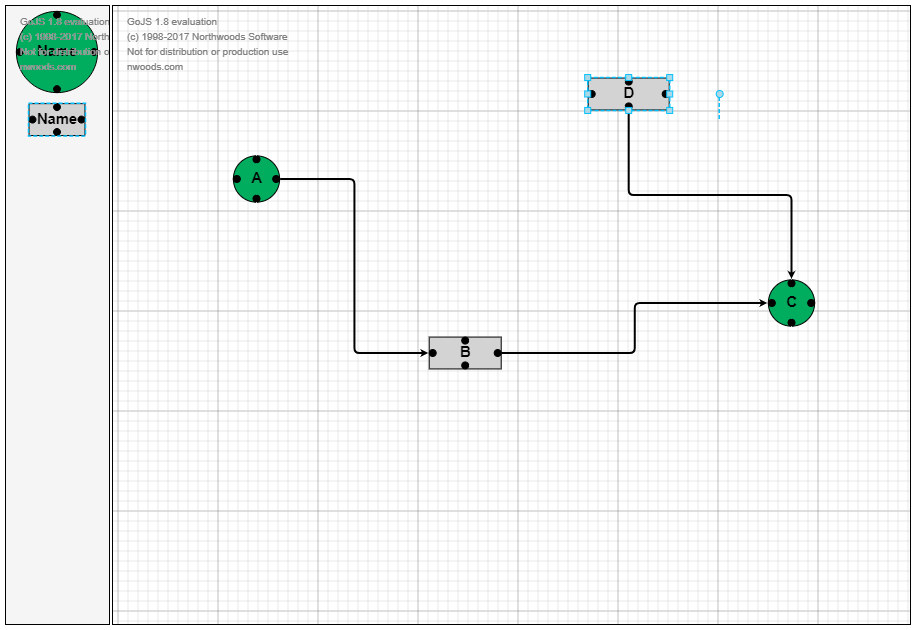
\includegraphics[scale=0.75]{gojssample.png}
	\caption{Ejemplo GoJS}\label{fig:gojssample}
\end{figure}

\vspace{5mm}

Para empezar, observando la figura anterior, cabe destacar que, para poder llevar a cabo este diagrama, es necesario reservar dos secciones del html (div). Una para la paleta de la izquierda contenedora de los elementos que son arrastrables, en este caso el círculo, y otro para el diagrama sobre el que se realizarán las acciones.


\vspace{5mm}

Para poder analizar detalladamente como se contruye a nivel Javascript la figura anterior, se irán explicando progresivamente los fragmentos del código que sean necesarios.

\vspace{5mm}

El elemento principal de esta estructura es el que contiene todo el resto y con el que posteriormente, en aplicaciones que integren el componente, se podrán comunicar, en este caso le llamaremos 'myDiagram'.

Lo principal de este diagrama es, como en todo lenguaje, darle un esqueleto, en GoJS los elementos adquieren dicha propiedad mediante la llamada a una librería de go llamada GraphObject bajo la sentencia make. Un ejemplo sencillo de creación de un diagrama sobre el espacio reservado del html llamado 'myDiagramDiv' es el siguiente:

\vspace{5mm}

\begin{figure}[H]
	\centering
	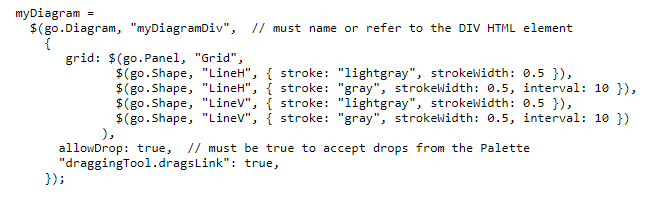
\includegraphics[scale=0.90]{creacionDiagramaGoJS.png}
	\caption{Creación Diagrama}\label{fig:creacionDiagramaGoJS}
\end{figure}

\vspace{5mm}

En la figura anterior se puede observar como se crea un diagrama. Además, se le asigna un grid o cuadrícula de fondo, así como, se le da la capacidad de poder arrastrar elementos sobre él.

\vspace{5mm}

Dentro del diagrama tambien se pueden crear declaraciones de variables y funciones. Un ejemplo concreto es el siguiente:

\begin{figure}[H]
	\centering
	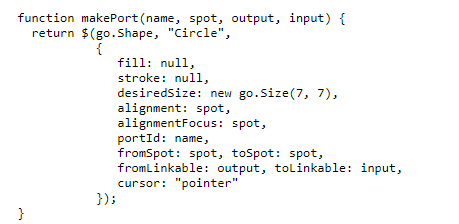
\includegraphics[scale=0.90]{funcionMakePort.png}
	\caption{Función MakePort}\label{fig:funcionMakePort}
\end{figure}

En este caso, se ha creado una función para crear puertos al círculo, estos puertos se usarán para enlazar los diferentes círculos entre sí, como se puede observar se declara toda la información tanto a nivel estético como a nivel de implementación. Esta función será utilizada posteriormente en la especificación del elemento círculo.

\vspace{5mm}

\begin{figure}[H]
	\centering
	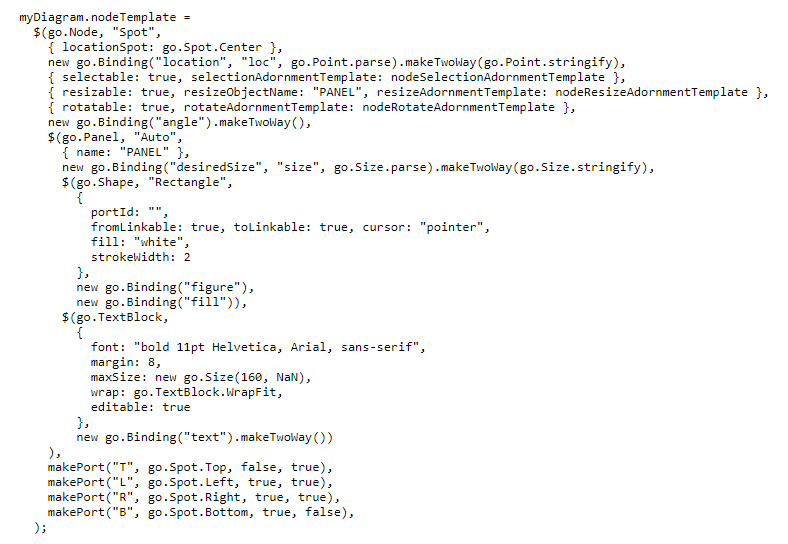
\includegraphics[scale=0.90]{nodeTemplate.png}
	\caption{Node Template}\label{fig:nodeTemplate}
\end{figure}
\vspace{5mm}

La imagen anterior describe una de las partes fundamentales, la especificación de los nodos, los nodos son todos aquellos elementos de los que se va a componer el diagrama, por lo tanto, hay que ser cautos a la hora de implementarlos.

\vspace{5mm}

Para este ejemplo, se va a crear un nodo círculo. Para ello lo primero es declarar el nodo con '\$(go.Node' seguido de todas las propiedades que le queramos especificar. En el ejemplo se le da una localización en el template\footnote{El template es el espacio que alberga, y sobre el que se definen las estructuras que definen un nodo.} y se le da las propiedades de poder ser seleccionado, redimensionado y rotado.

\vspace{5mm}

El template también se compone de un panel que de forma por defecto poseerá una forma rectangular que albergará un texto en su interior. Además, la sentencia 'new go.Binding' permite al usuario modificar una propiedad después de haber sido declarara en el template.

\vspace{5mm}

Por ultimo, se hacen cuatro llamadas a la función descrita anteriormente, que lo que hacen es crear cuatro puertos a cada lado del eje del círculo. En esta función se crea una figura circular junto con sus propiedades de enlazado.

\vspace{5mm}

\begin{figure}[H]
	\centering
	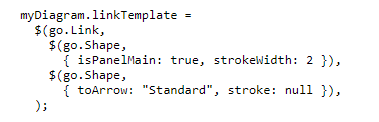
\includegraphics[scale=0.90]{linkTemplate.png}
	\caption{Link Template}\label{fig:linkTemplate}
\end{figure}
\vspace{5mm}

En esta figura se describe, al igual que la anterior, la información relativa al enlazado de los nodos. Esta vez, a los link solo se les establece un panel principal que define el tamaño del link, y otro panel secundario que establece la direccionalidad del link.

\vspace{5mm}

\begin{figure}[H]
	\centering
	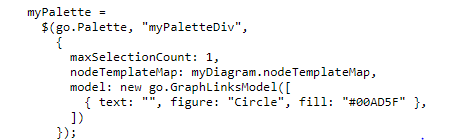
\includegraphics[scale=0.90]{palette.png}
	\caption{Paleta de Nodos}\label{fig:palette}
\end{figure}
\vspace{5mm}

Por último, esta figura describe la implementación de la paleta de nodos, o del conjunto de nodos que pueden ser arrastrados al diagrama para ser creados. Ésta se define bajo el mismo template que los nodos y se le añade al modelo de datos de la paleta un elemento círculo de color verde y sin texto en su interior.

\subsection{Conclusión}

GoJs es una herramienta que permite realizar una gran cantidad y combinación de figuras a nivel gráfico, además de proveer mecanismos para establecer una lógica de ejecución interna.